\documentclass{article}

% Chinese Support using xeCJK
% \usepackage{xeCJK}
% \setCJKmainfont{SimSun}

% Chinese Support using CTeX
\usepackage{ctex}

% Math Support
\usepackage{amsmath}
\usepackage{amsfonts}
\usepackage{amssymb}
\usepackage{wasysym}
\newcommand{\angstrom}{\text{\normalfont\AA}}
\usepackage{fancyhdr}

% Graphics Support
\usepackage{graphicx}
\usepackage{float}
\restylefloat{table}

% Reduced page margin
\usepackage{geometry}
\geometry{a4paper,scale=0.8}

\usepackage{caption}
\usepackage{subcaption}

% d and e should be math operators
\newcommand*{\dif}{\mathop{}\!\mathrm{d}}
\newcommand*{\md}{\mathop{}\!\mathrm{d}}
\newcommand*{\me}{\mathrm{e}}

% No indent for each paragraph
% \usepackage{parskip}
% \setlength{\parindent}{0cm}

% Bold style for Greek letters
\usepackage{bm}
\let\Oldmathbf\mathbf
\renewcommand{\mathbf}[1]{\boldsymbol{\Oldmathbf{#1}}}

% More space for dfrac in cell
\usepackage{cellspace}
\setlength{\cellspacetoplimit}{5pt}
\setlength{\cellspacebottomlimit}{5pt}

% SI units
\newcommand{\si}[1]{\  \mathrm{#1}}

% Multi-line author information
\usepackage{authblk}
\author{物理(4+4)1801 \quad  胡喜平 \quad U201811966}
\affil{个人网站 https://hxp.plus/ \quad 电子邮件 hxp201406@gmail.com}

\title{综合物理实验预习笔记——LabVIEW 使用基础}

\pagestyle{fancy}
\fancyhf{}
\lhead{源码地址:https://github.com/hxp-plus/Notes/tree/master/Physics-Experiment}
\rfoot{第 \thepage 页}
\renewcommand{\headrulewidth}{1pt}
\renewcommand{\footrulewidth}{1pt}

\begin{document}

\maketitle\thispagestyle{fancy}

\section{实验内容}

用LabVIEW虚拟仪器测量材料的磁滞现象和磁滞回线。

\section{实验原理}

\subsection{铁材料的磁滞现象}

将一个未磁化的铁放入磁场中进行磁化,初次磁化时磁感应强度和磁场的关系是曲线$\overline{ao}$,但是当磁场减为零后,铁内部的磁感应强度没有消失,磁感应强度和磁场强度的曲线是$\overline{ac}$,当磁场强度为零时,磁感应强度是$B_r$,当磁场强度为$-H_C$时,磁感应强度才降为零。
\begin{figure}[H]
  \centering
  \begin{subfigure}{0.48\linewidth}
    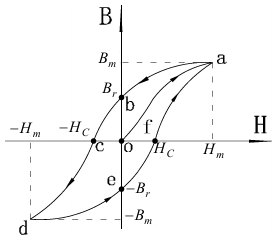
\includegraphics[width=\linewidth]{figures/磁滞现象1}
    \subcaption{单条磁滞回线}
  \end{subfigure}
  \begin{subfigure}{0.48\linewidth}
    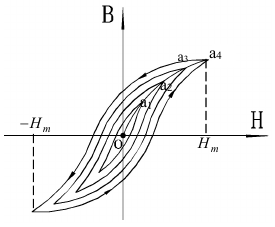
\includegraphics[width=\linewidth]{figures/磁滞现象2}
    \subcaption{一系列逐渐增大的磁滞回线}
  \end{subfigure}
  \caption{铁材料的磁滞现象}
\end{figure}

反复变化磁场,从$H_m$变化到$-H_m$,刚开始令$H_m$很小,之后逐渐增大$H_m$,可以发现磁化曲线越来越大,直到$H_m$足够大使得铁磁材料处于饱和状态。

\subsection{测量磁滞回线的实验装置原理}

下图是磁滞回线实验装置的原理图,用信号发生器给线圈加入变化的电流,从而产生变化的磁场。铁磁质里面的变化的磁感应强度产生电流,我们测量电流来测量铁磁质中的磁感应强度变化,之后积分得出铁磁质中的磁感应强度。

\begin{figure}[H]
  \centering
  \begin{subfigure}{0.38\linewidth}
    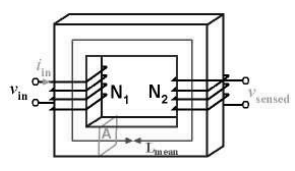
\includegraphics[width=\linewidth]{figures/磁滞回线装置-线圈}
    \subcaption{装置的线圈}
  \end{subfigure}
  \begin{subfigure}{0.58\linewidth}
    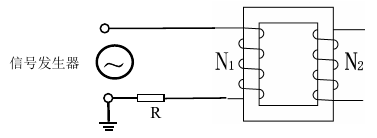
\includegraphics[width=\linewidth]{figures/磁滞回线装置-测量电路}
    \subcaption{测量实验结果的电路}
  \end{subfigure}
  \caption{磁滞回线测量实验装置}
\end{figure}

图中左边是输入右边是输出,分别用下标1和2表示。线圈有效长度为$L$,线圈匝数为$N_1$和$N_2$,线圈截面积$A$。

当信号发生器输入的电压产生的交变电流为$i_1$时,产生的磁场为

\begin{equation*}
  \begin{aligned}
    H = \frac{N_1 i_1}{L}
  \end{aligned}
\end{equation*}

其中产生的交变电流通过测量$R$两端的电压间接得到。产生的磁感应强度需要通过积分得到

\begin{equation*}
  \begin{aligned}
    B = \int \frac{v\md t}{N_2 A}
  \end{aligned}
\end{equation*}

其中$v$是感应电压。

\end{document} 


%%% Local Variables:
%%% mode: latex
%%% TeX-master: t
%%% End:
